In this section, we describe the overall approach we adopt in this thesis to create a benchmark of executable python software and using this benchmark to generate a data set for training a machine learning model for program analysis and further use this trained model to perform some of the machine learning tasks in program analysis.

The overall workflow of our approach is shown in the Figure \ref{fig:overall_approach}. In the section \ref{approach:selection of projects}, we describe the details on how we select specific projects from the large corpus of python projects. We describe the installation and setup of the selected projects in the section \ref{approach:setup and install}. In section \ref{approach:command line interface} we describe the command line interface and what can be done using it. In section \ref{approach:dynamic analysis} we describe the various dynamic analysis that we can perform to generate data set for program analysis. We describe the machine learning model and its training data in the section \ref{approach:ml model}. Finally, in section \ref{approach:application} we describe how we can use this framework and the trained machine learning model for program analysis.

\begin{figure}[ht]
\centering
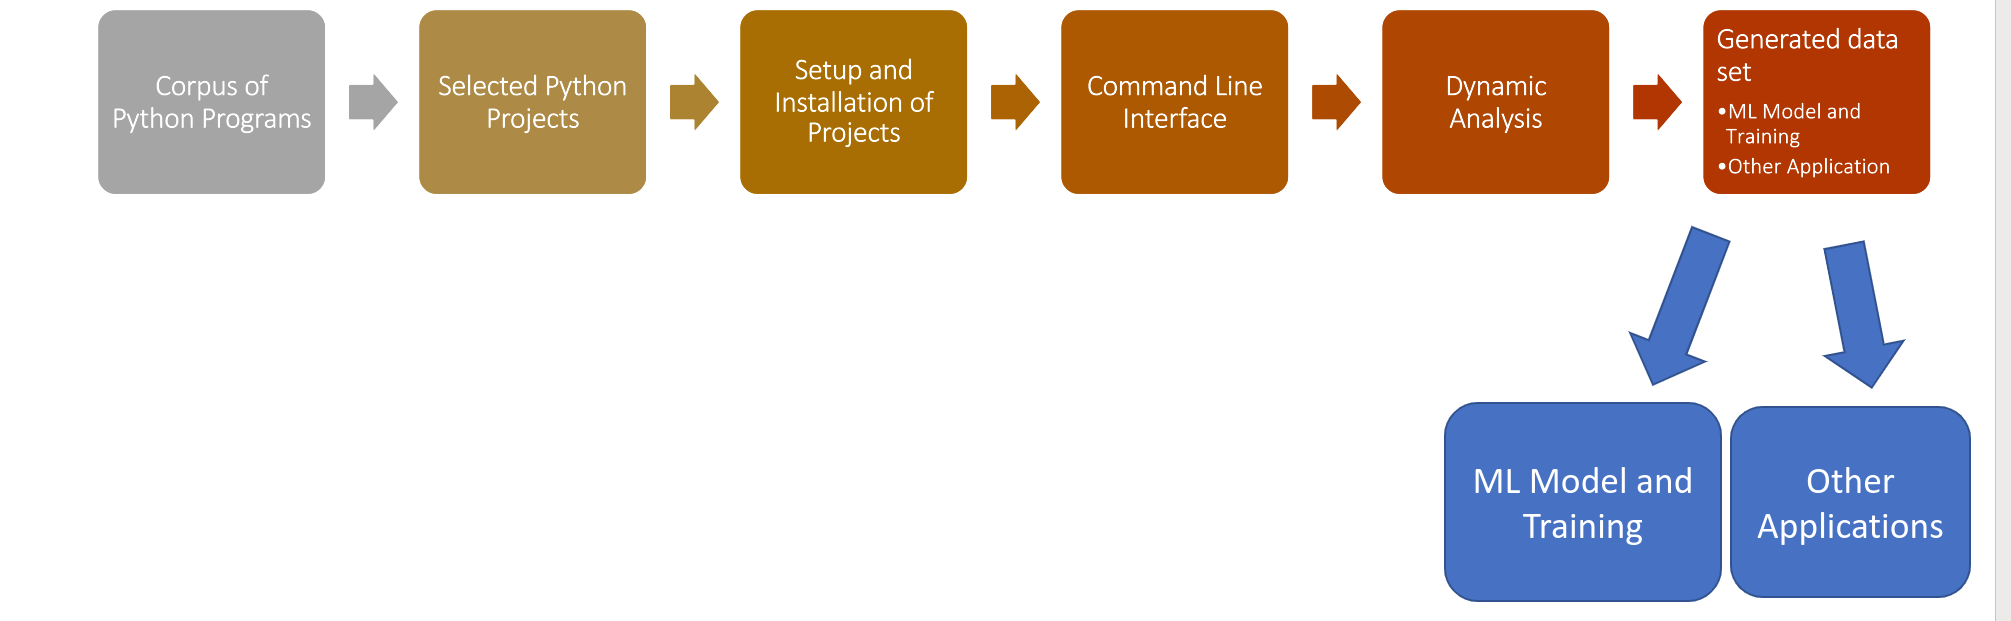
\includegraphics[width=1\linewidth]{figures/approach/Approach2.png}
\caption[Approach]{\label{fig:overall_approach}Overall Approach of DyPyBench.}
\end{figure}

\section{Selected Python Projects}
\label{approach:selection of projects}
Since Python is a very popular and general purpose programming language, it has been used in many domains and we have a large set of open source python projects available on the internet. In this thesis we target projects from many of these varied domains which are well accepted in the community and at the same time open sourced. Another important factor is the availability of test suites in the project source code. 

\section{Setup and Install}
\label{approach:setup and install}
With a set of selected projects based on the required criteria, we then proceed to setup and install these projects with each one having its own virtual environment to install all the dependencies with their specific version from the requirements file. And then also using the source to install the project and its dependencies with pip package manager. Each of these projects are numbered and are placed inside their own folders. The projects source is cloned to a particular date. We also install some of the other python packages using pip in order to run the test suites successfully. We end the setup with installing the packages for testing and analysis tools present in the benchmark.

\section{Command Line Interface}
\label{approach:command line interface}
With the selected projects from section \ref{approach:selection of projects} installed and setup, we provide a command line interface for the user to run tests and dynamic analysis of a single project or a collection of projects. This command line interface is a single command with various available options. The various options available are to list all the installed projects with their urls, run the test suite of the project, perform instrumentation of the source code for dynamic analysis using dynapyt or lexecutor. execution of lexecurtor or dynapyt analysis. It also provides the option to update dynapyt and lexecutor. WE can also store the output to a particular file or spefic a timeout for the specific tasks where applicable. 

\section{Dynamic Analysis}
\label{approach:dynamic analysis}
While the command line interface provides us with varied options, one such option is the dynamic analysis. There are two available analysis, dynapyt and lexeecutor. We can use the command line to perform the specific analysis and generate the logs which we can use to train machine learning models for program analysis or use these logs on our own to understand the behaviour of the selected projects. These analysis can also help us in discovering some issues in the selected python projects. An example is dynapyt which explored a bug in pytorch. 

\section{ML Model}
\label{approach:ml model}

\section{Application}
\label{approach:application}